\documentclass[12pt]{article}

\usepackage[T1]{fontenc}
\usepackage[scaled]{beramono}
%\usepackage{bera}
\usepackage{tikz}
\usetikzlibrary{shapes,arrows}
\usepackage{listings}
\usepackage{libertine}
\usepackage[T1]{fontenc}
\usepackage{MnSymbol}

\usepackage{color}
\definecolor{bluekeywords}{rgb}{0.13,0.13,1}
\definecolor{greencomments}{rgb}{0,0.5,0}
\definecolor{redstrings}{rgb}{0.9,0,0}

\definecolor{mygreen}{rgb}{0,0.6,0}
\definecolor{mygray}{rgb}{0.2,0.2,0.2}
\definecolor{mymauve}{rgb}{0.58,0,0.82}

\usepackage{listings}
\lstset{escapechar=\@}



% Define block styles
\tikzstyle{block} = [rectangle, draw, fill=blue!20, 
    text width=3.2em, text centered, rounded corners, minimum height=3em]
\tikzstyle{line} = [draw, -latex']
    

\title{02242: Program analysis \\ 
		\medskip \large{Technical University of Denmark} \\ \medskip  \large{First draft}}

\author{Ibrahim Nemli - s093477 \\
        Kim Rostgaard Christensen - s084283\\
        Peter Gammelgaard Poulsen - s093263}
\begin{document}
\maketitle
 
\begin{abstract}
This is the report documenting and describing the work done in the course 02242: Program Analysis.
\end{abstract}

\section{Introduction}
Program analysis is the discipline of extracting and deriving information about the structure, and potential behaviour of computer programs. It has many applications, such as; bug finding, optimizations, code reuse, formal validation and model mapping. In this report, we take a closer look at some of the specialized and general theory used for transforming source code text into analysis-friendly structures, and then performing the actual analysis on them.

\section{Program representation}
The first problems we need to solve is which data structures should be used for our abstract syntax tree, which will serve as the first step of our intermediate representation.
\subsection*{(a) Abstract syntax tree data structure}
We have decided that we could use an unbalanced tree for storage of our abstract syntax tree in our target programming language.
\subsection*{(b) Flow graph data structure}
%Present a data structure for flow graphs and give an algorithms for transforming abstract syntax trees into flow graphs.
This is a typical tree structure, with a parent reference.
\subsection*{(c) Program graph data structure}
Present a data structure for program graphs and give an algorithm for
transforming abstract syntax trees into program graphs.


\section*{**Notes Below**}

\subsection*{Constructing flow graphs}

\begin{description}
   \item[Functions:] Slide 11+12 of from week 2
   \item[label(S):] The set of nodes of the flow graph S
   \item[Init(S):] The initial node of the flow graph S. Unique node where the execution of the program starts.
   \item[Final(S):] The final node of the flow graph S. A set of nodes where the execution of the program may terminate.
   \item[Block(S):] A set of the blocks/statements in the program under inquisition.
   \item[Flow(S):] The edges of the flow graph for S. A set of pairs is returned.
\end{description}

\begin{figure}
\begin{lstlisting}
[y:=x]@$^1$@
[z:=1]@$^2$@
while [x>0]@$^3$@ do
   [z:= z*y]@$^4$@
   [Y:= y-1]@$^5$@
od
[y:=0]@$^6$@
\end{lstlisting}
\label{source:example1}
\caption{Source code example}
\end{figure}

\begin{figure}

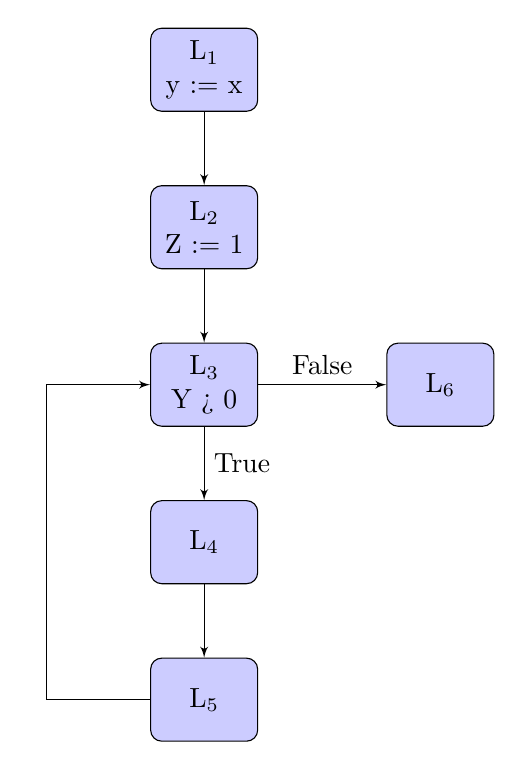
\begin{tikzpicture}[node distance = 2cm, auto]

    % Place nodes
    \node [block] (L1) {L$_1$ \\ y := x};
    \node [block, below of=L1] (L2) {L$_2$ \\ Z := 1};
    \node [block, below of=L2] (L3) {L$_3$ \\ Y > 0};
    \node [block, below of=L3] (L4) {L$_4$ \\ };
    \node [block, below of=L4] (L5) {L$_5$ \\};
    \node [block, right of=L3, node distance=3cm] (L6) {L$_6$ \\};

    % Draw edges
    \path [line] (L1) -- (L2);
    \path [line] (L2) -- (L3);
    \path [line] (L3) -- node {True} (L4);
    \path [line] (L3) -- node {False} (L6);
    \path [line] (L4) -- (L5);
   	\path [line] (L5) -| (-2,-6) |-  node [near start, color=black] {} (L3);

\end{tikzpicture}

\caption{Flow Graph}

\end{figure}

\begin{description}
\item[Label($S$):] $\left\lbrace   1,2,3,4,5,6   \right\rbrace$
\item[Initial($S$):] 1
\item[Final($S$):] $\left\lbrace   6   \right\rbrace$
\item[Blocks($S$):]$\{$ y:=x, z:=1 y>0, z:=z*y, y;=y-1, Y:=0 $\}$
\item[Flow($S$):] $\{ (1,2), (2,3), (3,4), (4,5), (5,3), (3,6) \}$
\end{description}

\subsection*{Constructing program graph}
Functions: Slide 14, week 2.\\
$pg^{qt}_{qs}$: The program graph for statement $S$ with with initial node being $q_{s}$\footnote{$s$ for source.}, and $q_{t}$\footnote{$t$ for target.}\\
Nodes are constructed by the algorithm.\\
The edges are represented by the tuple $(q_s, x, q_T)$ where $q_s$ and $q_t$ are nodes, and x is and elementary block statement. %NOTE, krc: shouldn't x be s ?

\begin{figure}[h]
\centering
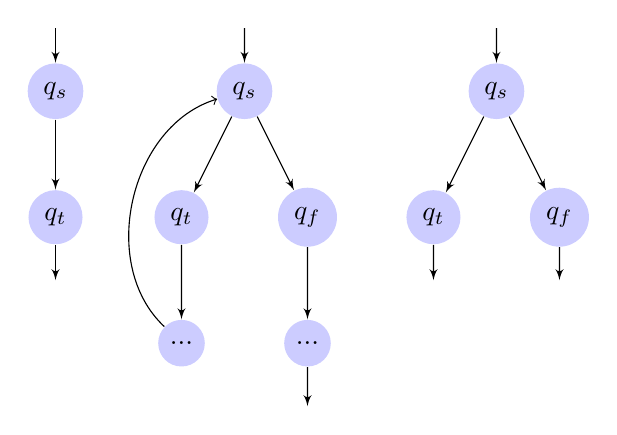
\begin{tikzpicture}
  [scale=.8,auto=left,every node/.style={circle,fill=blue!20}]
  \tikzstyle{line} = [draw, -latex']
  %\node (l1) [circle, draw=black, fill=white!20, text=black, scale=0.8]{$l_1$};
  \node (q_s) at (0,3)  {$q_s$};
  \node (q_t) at (0,1)  {$q_t$};

  \path [line] (0,4) -- (q_s);
  \path [line] (q_s) -- (q_t); %TODO; Add label here.
  \path [line] (q_t) -- (0,0);


  \node (q_s) at (3,3)  {$q_s$};
  \node (q_t) at (2,1)  {$q_t$};
  \node (q_f) at (4,1)  {$q_f$};
  \node (empty1) at (2,-1)  {$...$};
  \node (empty2) at (4,-1)  {$...$};

  \path [line] (3,4) -- (q_s);
  \path [line] (q_s) -- (q_t); %TODO; Add label here.
  \path [line] (q_s) -- (q_f); %TODO; Add label here.
  \path [line] (q_f) -- (empty2);
  \path [line] (q_t) -- (empty1);
  \path [line] (empty2) -- (4,-2);
  \draw[bend left=60,->]  (empty1) to (q_s);
  
  \node (q_s) at (7,3)  {$q_s$};
  \node (q_t) at (6,1)  {$q_t$};
  \node (q_f) at (8,1)  {$q_f$};

  \path [line] (7,4) -- (q_s);
  \path [line] (q_s) -- (q_t); %TODO; Add label here.
  \path [line] (q_s) -- (q_f); %TODO; Add label here.
  \path [line] (q_t) -- (6,0);
  \path [line] (q_f) -- (8,0);

\end{tikzpicture}
 \caption{Assignments, loops and branches}

 \label{fig:graph}
\end{figure}

%TODO Figure from 6.jpg

\begin{description}
\item[Label($S$):] $\{ 1,2,3,4,5,6,7 \}$
\item[Initial($S$):] $1$
\item[Final($S$):] $\{ 7 \}$
\item[Blocks($S$):]$\{ [y:=x], [z:=1], [y>0], [z:=z*y], [y;=y-1], [\lnot (y>0)] ,[Y:=0] \}$
\item[Flow($S$):] $\{ (1,2), (2,3), (3,4), (4,5), (5,3), (3,6), (6,7) \}$
\end{description}

$a_{\bullet}, a_{\circ}$

\section*{Enumerations}
\begin{verbatim}
Variable_Enum : {int, Array}
Operator_A_Enum : {Plus, Minus, Divide, Multiply}
Operator_R_Enum : {Less, Less_Equal, Equal, 
                   Not_Equal, Greater, Greater_Equal}
Operator_B_Enum : {And, Or}
\end{verbatim}


\section*{Exercise 2 - Program Slicing}

\subsection*{(a) Example program}
\begin{figure}
\begin{lstlisting}
program
[int x]@$^1$@
[int y]@$^2$@
[int <]@$^3$@
[y := x]@$^4$@
[z := 1]@$^5$@
while [y>0]@$^6$@ do
   [z:= z*y]@$^7$@
   [Y:= y-1]@$^8$@
od
[y:=0]@$^9$@
end
\end{lstlisting}
\label{source:example2}
\caption{Slicing code example}
\end{figure}

The point of interest is label 8.  The result of program slice analysis is; [y:=x]$^4$, [y:=y-1]$^8$, [int x]$^1$.\\\\

The point of interest is label 7.  The result of program slice analysis is; [y:=x]$^4$, [z:=1]$^5$, [z:=z*y]$^7$, [int z]$^3$, [int y]$^2$.\\\\



\begin{table}[h]
    \begin{tabular}{l | l }
    \textbf{int x} &  kill$_{RD}$([int x]$^2$) = $\emptyset$ \\
                   &  gen$_{RD}$([int x]$^2$) = $\{(x,2)\}$ \\
    \hline
    \textbf{A[n]} & kill$_{RD}$([A[n]]$^2$) = $\emptyset$\\
                  & gen$_{RD}$([A[n]$^2$) = $\{(A[0],l), ... (A[i-a],l)\}$ \\

    \hline
    \textbf{A[a$_1$ := a$_2$} & kill$_{RD}$([A[a$_1$]]$^2$) = \{ (A[a$_1$],l' \} \\
                              & gen$_{RD}$([A[n]$^2$) = $\{(A[0],l), ... (A[i-a],l)\}$ \\

    \end{tabular}
    \centering
	\caption{RD Equations}
	\label{table:rd_equations}
\end{table}


\paragraph*{:}

\paragraph*{int A[n]:}


\subsection*{(b) Extending Reaching Definitions Analysis table}
\subsection*{(c) Flow graph}
\subsection*{(d) Program slice calculation algorithm}
\section*{Exercise 3}

Where 

\section*{Exercise 4 - Buffer overflow}
\begin{equation}
  \left(L, \mathcal{F}, F, E, \iota, \mathrm{f}.  \right)
  \label{eq:monotone_framework}
\end{equation}
%TODO: Put this into a table.
We define our complete lattice to; $(?,\sqsubseteq,\bigsqcup, \bigsqcap, \top, \bot )$, and our interval is defined to: Interval = $\{\bot\} \bigcup \{[Z_2, Z_2] | Z_1 < Z_2, Z_1, Z_2, \in Z' \bigcup \{- \infty, \infty \} \} $, where $Z' = \{ Z | \min \leq Z \leq \max \}$ and $ - \infty \leq \infty $ minimum $ \in Z$\\
$\sqsubseteq$-Ordering: $\subseteq$ (subset ordering).\\
Interval$_1 \sqsubseteq $ Interval$_2 $ if, and only if $\beta($Interval$_1) \subseteq \beta($Interval$_2)$, where $\beta(\bot) = \emptyset$\\
%TODO $\beta([Z_1, Z_2]) = \emptyset$
Least upper bound: $\bigsqcup Y = \bigcup Y$\\
Greatest lower bound: $\bigsqcap Y = \bigcap Y$\\
$\bot$ : Bottom, least element : $\emptyset$\\
$\top$ : Top, greatest element : $[-\infty, \infty]$\\\

This is a complete lattice, as every subset in the partial ordered set have a least upper bound and a greatest lower bound.\\
It also holds the Ascending Chain Property, because the lattice has a finite height, and will thus, eventually stabilize.


\subsection*{Internal analysis}

\end{document}